\documentclass{sprz}

\addbibresource{bibliography.bib}

% Hiperlinki w PDF (spis treści, odwołania, cytowania, URL)
\usepackage[hidelinks]{hyperref}
\usepackage{bookmark}
\graphicspath{{img/}}

% =============================================================================
% Dane osobowe / formalne
% =============================================================================
\studfield{Informatyka}
\studtype{Stacjonarne}
\title{RacePortal --- platforma wydarzeń motorsportowych}
\engtitle{RacePortal --- a platform for motorsports events}
\acronym{RP}
\titledate{2025-10-01}
\supervisor{dr hab.\ Marek Bendarczyk}
\reviewer{mgr Alex Polin}
\author{Otrombke Natalia}{s26828}{Cyberbezpieczeństwo}{Stacjonarny}
\author{Kasprowicz Oliwier}{s30290}{Cyberbezpieczeństwo}{Stacjonarny}
\author{Gutowski Michał}{s30572}{Cyberbezpieczeństwo}{Stacjonarny}
\author{Parkitny Miłosz}{s30287}{Cyberbezpieczeństwo}{Stacjonarny}
\author{Wronisz Wojciech}{s26999}{Cyberbezpieczeństwo}{Stacjonarny}
\consultant{--- brak ---}
\projectgoals{Celem projektu jest zaprojektowanie i~zaimplementowanie systemu RacePortal --- centralnego katalogu wydarzeń motorsportowych w~Polsce, umożliwiającego przeglądanie wydarzeń (lista, mapa, kalendarz), zarządzanie garażem pojazdów, zgłoszenia udziału oraz obsługę ról organizatora i~administratora, wraz z~aplikacją mobilną typu wizytówka oraz konteneryzowanym środowiskiem uruchomieniowym.}
\productsandservices{Aplikacja webowa (React/Vite), API REST (Spring Boot) z~bazą MySQL, aplikacja mobilna Expo (katalog wydarzeń z~CTA do weba), wspólne typy API (\texttt{packages/api-types}), dokumentacja projektowa oraz zestaw testów automatycznych (JUnit, Vitest, Playwright).}
\mainfunctionalities{Katalog wydarzeń z~filtrami oraz widokami lista/mapa/kalendarz; szczegóły wydarzenia i~wyznaczanie trasy (OSRM); konta użytkowników (JWT, RBAC); garaż pojazdów i~dopasowanie kategorii do wydarzenia (\texttt{carMatch}); system zgłoszeń ze statusami i~powiadomieniami e-mail; panele organizatora i~administratora; archiwum; mobilna wizytówka z~przekierowaniem zapisu na web.}
\successmeasure{Działający stos Docker Compose (web, API, MySQL, Mailpit, backup); realizacja funkcji MVP katalogu, zapisów i~ról; pozytywne wyniki testów automatycznych API/web/mobile unit; możliwość demonstracji pełnego scenariusza: gość $\rightarrow$ kierowca $\rightarrow$ organizator $\rightarrow$ administrator oraz mobilka $\rightarrow$ CTA web.}
\projlimitations{Brak natywnej bramki płatności (PSP); upload plików zastąpiony adresami URL; aplikacja mobilna bez pełnej parity z~webem (świadoma wizytówka); brak publikacji w~sklepach App Store/Google Play; brak formalnego testu obciążenia 10k rekordów / 50~RPS; produkcyjny TLS poza domkniętym zakresem lokalnego MVP (w~prod: Cloudflare Tunnel).}
\date{miesiąc, rok obrony} % TODO
\finishdate{\today}
\nabstract{Praca przedstawia projekt i~implementację systemu RacePortal --- platformy wspierającej katalogowanie wydarzeń motorsportowych oraz proces zapisów uczestników. System obejmuje aplikację webową, backend REST oparty o~Spring Boot i~MySQL oraz aplikację mobilną Expo pełniącą rolę publicznej wizytówki katalogu. W~pracy opisano problem dziedzinowy, wymagania, architekturę, realizację kluczowych modułów (wydarzenia, garaż, zgłoszenia, role), mechanizmy bezpieczeństwa (JWT, RBAC) oraz weryfikację testami automatycznymi. Wynikiem jest działające, konteneryzowane środowisko demonstracyjne zgodne z~zakresem MVP projektu.}
\keyword{motorsport}
\keyword{katalog wydarzeń}
\keyword{system zapisów}
\keyword{zarządzanie wydarzeniami}
\keyword{aplikacja mobilna}



\begin{document}

\maketitle

\makeprojectcard

\makedeclarationsai

\tableofcontents

\chapter{Informacje wstępne}
\section{Cel i zakres pracy}
Celem pracy jest zaprojektowanie oraz implementacja systemu \textbf{RacePortal} --- platformy internetowej (z~uzupełnieniem mobilnym) służącej jako centralny katalog wydarzeń motorsportowych w~Polsce oraz narzędzie do obsługi zapisów kierowców.

Zakres obejmuje:
\begin{itemize}
  \item aplikację webową (katalog, konta, garaż, zgłoszenia, panele organizatora i~administratora);
  \item API REST z~trwałą bazą danych wydarzeń, użytkowników i~zgłoszeń;
  \item powiadomienia e-mail (potwierdzenia, statusy, weryfikacja konta);
  \item mapę wydarzeń oraz wyznaczanie trasy dojazdu (OSRM; opcjonalnie Google Maps przy kluczu API);
  \item aplikację mobilną Expo jako \emph{wizytówkę} katalogu z~CTA zapisu na stronie webowej;
  \item konteneryzację (Docker Compose) oraz podstawowy zestaw testów automatycznych.
\end{itemize}

Poza zakresem MVP pozostają m.in.\ natywne płatności online, pełny upload plików binarnych, push notifications oraz publikacja aplikacji mobilnej w~sklepach.

\section{Wizja rozwiązania}
\label{sec:wizja}
RacePortal ma być \textbf{jednym miejscem} odkrywania i~obsługi startów motorsportowych w~Polsce: kierowca znajduje wydarzenie, sprawdza wymagania względem własnego garażu i~składa zgłoszenie; organizator publikuje imprezę i~zarządza listą uczestników; administrator moderuje treści i~role.

Wizja produktowa zakłada:
\begin{itemize}
  \item publiczny katalog z~trzema widokami (lista, mapa, kalendarz) na wspólnych filtrach;
  \item ujednolicony proces zapisu ze statusami i~powiadomieniami e-mail;
  \item wyraźny podział ról \texttt{USER} / \texttt{ORGANIZER} / \texttt{ADMIN} (gość przegląda bez konta);
  \item mobilną ścieżkę discovery (Expo) z~konwersją zapisu na web;
  \item uruchamialne środowisko demonstracyjne (Docker) oraz wdrożenie produkcyjne za Cloudflare Tunnel.
\end{itemize}

Szczegóły warstw technicznych (web React/Vite, API Spring Boot, MySQL, mobile Expo, \texttt{packages/api-types}) opisano w~rozdziale~\ref{ch:projekt} oraz w~rozdziałach implementacyjnych. Kod źródłowy utrzymywany jest w~repozytorium projektu~\cite{raceportal:repo}.

\section{Struktura pracy}
Kolejne rozdziały obejmują: słownik pojęć, opis problemu dziedzinowego, kontekst biznesowy (w~tym karty udziałowców), analizę SWOT, planowanie projektu, analizę wymagań (w~tym karty wymagań i~diagramy UML), projekt systemu (m.in.\ Figma, diagram klas), opis realizacji oraz szczegóły implementacji backendu, frontendu i~mobile, bezpieczeństwo, testowanie, prezentację systemu, nakład pracy, \textbf{wkład własny} oraz podsumowanie (z~uwzględnieniem ograniczeń wydajnościowych RPS).

\chapter{Słownik pojęć}
\begin{description}
  \item[Wydarzenie (event)] Zorganizowany start / impreza motorsportowa (np.\ track day, drift, rally), opisana datą, lokalizacją, kategorią i~wymaganiami.
  \item[Katalog] Publiczny wykaz wydarzeń z~widokami lista, mapa i~kalendarz oraz filtrami.
  \item[Garaż] Zbiór pojazdów przypisanych do konta kierowcy, wykorzystywanych przy zapisie na wydarzenie.
  \item[Zgłoszenie (registration)] Wniosek o~udział w~wydarzeniu, posiadający status (np.\ PENDING, APPROVED, CANCELED).
  \item[carMatch] Mechanizm dopasowania kategorii/klasy pojazdu do kategorii wydarzenia (aliasy nazw).
  \item[Organizator] Użytkownik z~rolą ORGANIZER, uprawniony do tworzenia i~zarządzania własnymi wydarzeniami oraz zgłoszeniami.
  \item[Administrator] Użytkownik z~rolą ADMIN, moderujący wydarzenia, wnioski o~rolę organizatora i~role kont.
  \item[Wizytówka mobilna] Wersja aplikacji Expo ograniczona do przeglądania katalogu; zapis odbywa się na webie (CTA).
  \item[JWT] JSON Web Token --- token sesji używany do uwierzytelniania żądań API.
  \item[RBAC] Role-Based Access Control --- kontrola dostępu oparta o~role.
  \item[OSRM] Open Source Routing Machine --- publiczny serwis wyznaczania trasy wykorzystany jako domyślny provider.
  \item[MVP] Minimum Viable Product --- minimalny zakres funkcji przyjęty do odbioru projektu.
  \item[RPS] Requests Per Second --- metryka obciążenia (np.\ docelowy test 50~RPS przy 10k rekordach).
\end{description}

\chapter{Opis problemu}
\section{Charakterystyka rynku wydarzeń motorsportowych}
% TODO: rozwinąć na podstawie pitch / research
Amatorski i~półprofesjonalny motorsport w~Polsce obejmuje liczne formy aktywności (track day, drift, rally, wyścigi górskie itp.). Informacje o~terminach i~zapisach są często rozproszone pomiędzy strony organizatorów, media społecznościowe oraz komunikatory.

\section{Problemy związane z~organizacją wydarzeń i~zapisami uczestników}
Organizatorzy potrzebują narzędzia do publikacji wydarzenia, zbierania zgłoszeń, weryfikacji wymagań wobec pojazdu/kierowcy oraz komunikacji statusu zgłoszenia. Ręczne procesy (arkusze, wiadomości prywatne) są podatne na błędy i~trudne do skalowania.

\section{Problemy informacyjne po stronie kierowców i~organizatorów}
Kierowcy mają trudność ze znalezieniem aktualnych startów w~jednym miejscu, porównaniem wymagań wydarzenia z~posiadanym pojazdem oraz śledzeniem statusu zapisu. Organizatorzy --- z~utrzymaniem spójnej listy uczestników i~powiadomień.

\section{Uzasadnienie potrzeby stworzenia systemu RacePortal}
RacePortal odpowiada na potrzebę \textbf{centralnego katalogu} oraz \textbf{ujednoliconego procesu zapisu} z~rolami użytkowników, przy zachowaniu prostego uruchomienia demonstracyjnego (Docker) i~ścieżki mobilnej (odkrywanie wydarzeń).

\section{Aspekty techniczne i~organizacyjne problemu}
Wyzwania obejmują: spójny model danych wydarzeń i~zgłoszeń, bezpieczeństwo kont (JWT, RBAC), walidację wymagań wydarzenia względem garażu, integrację mapy/trasy, dostarczalność maili w~środowisku deweloperskim oraz świadomy podział odpowiedzialności web vs mobile.

\chapter{Kontekst biznesowy}
\label{ch:biznes}
\section{Segmentacja użytkowników}
\begin{itemize}
  \item \textbf{Gość} --- przegląda katalog bez konta.
  \item \textbf{Kierowca (USER)} --- garaż, zapisy, profil.
  \item \textbf{Organizator} --- tworzy wydarzenia, zarządza zgłoszeniami.
  \item \textbf{Administrator} --- moderacja, role, wnioski o~organizatora.
\end{itemize}

Wczesny podział funkcjonalności według ról przedstawia rys.~\ref{fig:podzial-rol}.

\begin{figure}[ht]
  \centering
  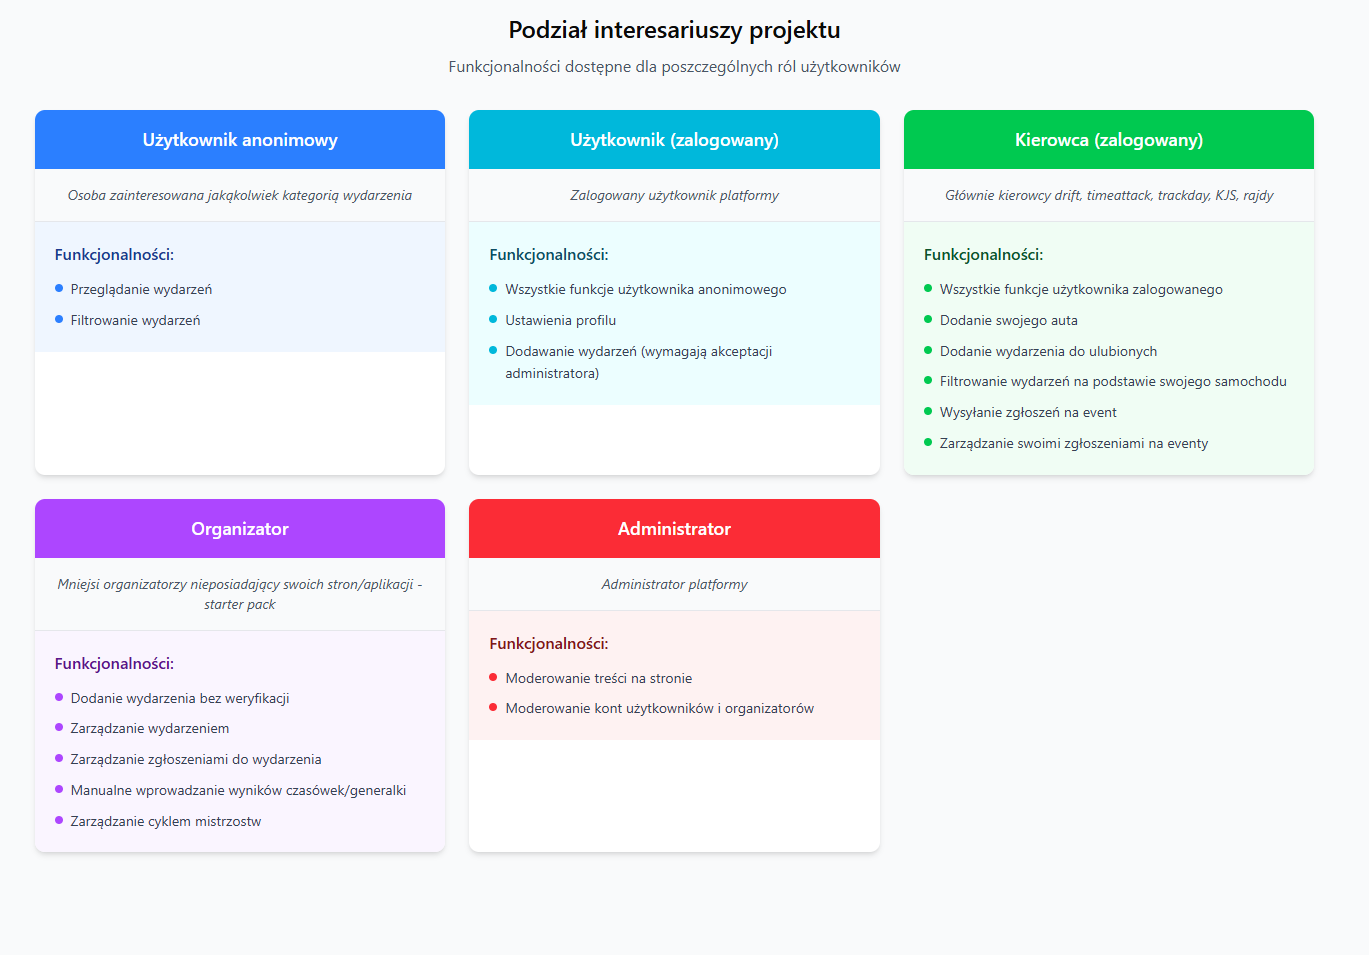
\includegraphics[width=\textwidth]{podzial-funkcjonalnosci.png}
  \caption{Podział interesariuszy projektu --- funkcjonalności dostępne dla ról użytkowników (materiał koncepcyjny).}
  \label{fig:podzial-rol}
\end{figure}

\section{Interesariusze systemu}
\label{sec:interesariusze}
Poniżej karty udziałowców (środowisko \texttt{stakeholder} szablonu PJATK). Odwołania do wymagań i~projektu wskazują rozdziały~\ref{ch:wymagania}--\ref{ch:projekt}.

\begin{stakeholder}[caption={Karta udziałowca: Kierowca},label={tab:ud-kierowca}]
\id{U-01}
\name{Kierowca (USER)}
\descr{Użytkownik z~kontem, który utrzymuje garaż pojazdów i~składa zgłoszenia na wydarzenia motorsportowe.}
\type{Użytkownik końcowy / klient platformy}
\viewpoint{Chce szybko znaleźć starty, dopasować auto do wymagań i~śledzić status zgłoszenia.}
\limitations{Zapis i~garaż wymagają konta web; mobilka w~MVP jest wizytówką bez pełnej parity.}
\requ{Wymagania funkcjonalne katalogu, garażu i~zgłoszeń --- rozdz.~\ref{ch:wymagania}; panel użytkownika --- rozdz.~\ref{ch:frontend}.}
\end{stakeholder}

\begin{stakeholder}[caption={Karta udziałowca: Organizator},label={tab:ud-organizator}]
\id{U-02}
\name{Organizator (ORGANIZER)}
\descr{Podmiot publikujący wydarzenia i~zarządzający listą zgłoszeń uczestników.}
\type{Dostawca treści / partner biznesowy}
\viewpoint{Potrzebuje prostego CRUD wydarzeń, weryfikacji zgłoszeń i~komunikacji statusów (e-mail).}
\limitations{MVP bez natywnej bramki płatności (PSP); dowód płatności jako URL.}
\requ{Panel organizatora i~RBAC --- rozdz.~\ref{ch:wymagania}, \ref{ch:projekt}; implementacja --- rozdz.~\ref{ch:backend}.}
\end{stakeholder}

\begin{stakeholder}[caption={Karta udziałowca: Administrator},label={tab:ud-admin}]
\id{U-03}
\name{Administrator (ADMIN)}
\descr{Operator platformy moderujący wydarzenia, role kont oraz wnioski o~uprawnienia organizatora.}
\type{Właściciel / operator systemu}
\viewpoint{Zapewnia jakość katalogu i~bezpieczeństwo ról bez ręcznej ingerencji w~bazę.}
\limitations{Skala produkcyjna (RODO operacyjne, WAF, 2FA) poza zakresem MVP demonstracyjnego.}
\requ{Panel admina, bezpieczeństwo JWT/RBAC --- rozdz.~\ref{ch:bezpieczenstwo}; testy RBAC --- rozdz.~\ref{ch:testy}.}
\end{stakeholder}

\section{Propozycja wartości systemu}
Jedno miejsce na odkrywanie startów, dopasowanie auta do wymagań wydarzenia i~obsługę statusu zgłoszenia --- z~osobnymi narzędziami dla organizatora i~administratora.

\section{Kanały komunikacji i~dystrybucji}
Aplikacja webowa jako kanał główny (\url{https://raceportal.pl}); e-mail (Mailpit w~dev, Mailbux w~prod); mobilna wizytówka jako kanał discovery z~konwersją na web; repozytorium GitHub jako kanał dystrybucji kodu.

\section{Kluczowe zasoby i~działania}
Zespół deweloperski, infrastruktura Docker, seed danych demo, dokumentacja (\texttt{docs/}), scenariusze prezentacji i~testy automatyczne.

\section{Model działania platformy}
Platforma pośredniczy między organizatorami (podaż wydarzeń) a~kierowcami (popyt na starty). Na etapie MVP nie rozlicza płatności --- obsługuje statusy zgłoszeń i~dowód płatności jako URL.

\section{Realistyczność wdrożenia i~dalsze perspektywy}
Lokalne MVP jest uruchamialne na stacji deweloperskiej. Wdrożenie produkcyjne zrealizowano na Oracle Always Free z~tunelowaniem Cloudflare (TLS i~DNS po stronie Cloudflare) --- szczegóły w~rozdz.~\ref{sec:arch-fizyczna}. Dalsze perspektywy: PSP, upload plików, push, publikacja mobile w~sklepach.

\section{Kontekst prawny i~etyczny}
System przetwarza dane konta (e-mail, opcjonalnie dane profilu). W~UI uwzględniono politykę prywatności oraz notę RODO przy tworzeniu wydarzenia. Pełna zgodność procesowa (DPIA, retencja) wykracza poza demonstracyjne MVP.

\chapter{Analiza SWOT}
\section{Mocne strony (Strengths)}
\begin{itemize}
  \item Pełny przepływ ról: gość, kierowca, organizator, administrator.
  \item Trzy widoki katalogu na wspólnych filtrach (lista / mapa / kalendarz).
  \item Konteneryzacja i~seed kont demonstracyjnych ułatwiają prezentację.
  \item Testy automatyczne (API, web E2E, unit mobile / api-types).
  \item Wspólne typy API ograniczają dryf web~$\leftrightarrow$~mobile.
\end{itemize}

\section{Słabe strony (Weaknesses)}
\begin{itemize}
  \item Brak prawdziwego uploadu plików i~bramki płatności.
  \item Mobilka bez logowania i~garażu (wizytówka).
  \item Zależność od publicznych serwisów map/trasy (CARTO/OSRM).
  \item Częściowe rozjazdy względem wewnętrznej Specyfikacji Formularzy.
  \item Brak formalnego testu obciążenia 10k rekordów / 50~RPS.
\end{itemize}

\section{Szanse (Opportunities)}
\begin{itemize}
  \item Rozszerzenie o~PSP, waitlistę, watchlistę i~eksport list startowych.
  \item Integracje z~kalendarzami (iCal) i~powiadomienia push.
  \item Budowa społeczności wokół torów i~organizatorów regionalnych.
\end{itemize}

\section{Zagrożenia (Threats)}
\begin{itemize}
  \item Konkurencja ze strony grup społecznościowych i~dedykowanych systemów zapisów.
  \item Zmiany limitów / dostępności publicznych API map i~routingu.
  \item Wymogi RODO i~odpowiedzialność za dane osobowe przy skali produkcyjnej.
\end{itemize}

\chapter{Planowanie projektu}
\section{Cele projektu}
Dostarczenie działającego MVP katalogu i~zapisów z~rolami użytkowników, mapą, mailami, mobilną wizytówką oraz dokumentacją i~testami umożliwiającymi odbiór / prezentację.

\section{Zakres projektu}
Zgodnie z~listą funkcji MVP 1--15 (katalog, filtry, detal, admin, konto, garaż, zgłoszenia, organizator, baza, maile, mapa, trasa, archiwum, mobile) --- szczegóły w~dokumentacji projektowej \texttt{docs/MVP.md}.

\section{Metodyka pracy}
Iteracyjne dostarczanie funkcji w~monorepo, z~bieżącą dokumentacją zmian (\texttt{docs/changes.md}) oraz weryfikacją testami po istotnych zmianach.

\section{Organizacja zespołu}
Zespół pięcioosobowy pracuje we wspólnym repozytorium Git, z~podziałem na warstwy web / API / mobile / dokumentacja / diagramy. Szczegółowy opis wkładu --- rozdz.~\ref{ch:wklad}.

\section{Harmonogram pracy}
% TODO: uzupełnić datami kamieni milowych zespołu
Prace obejmują m.in.\ prototyp Figma Make, scaffold UI, implementację backendu Spring, parity funkcji web, testy, uproszczenie mobile do wizytówki, wdrożenie Oracle + Cloudflare Tunnel oraz domykanie dokumentacji odbiorczej.

\section{Infrastruktura i~środowisko pracy}
Docker Desktop, Node.js (web/mobile), JDK/Maven (API w~kontenerze), Expo / iOS Simulator lub Android Emulator, Playwright, GitHub, Cloudflare Tunnel (\texttt{cloudflared}), Oracle Cloud VM.

\section{Analiza ryzyka projektowego}
\subsection{Analiza zagrożeń}
\begin{itemize}
  \item Niespójność wymagań formularzy vs implementacja --- mitigacja: rejestr luk (\texttt{spec-conformity.md}).
  \item Awaria zewnętrznego OSRM/CARTO --- mitigacja: graceful fallback komunikatów, możliwość wymiany providera.
  \item Dryf typów web/mobile --- mitigacja: \texttt{packages/api-types}.
  \item Opóźnienia wynikające z~rozrostu zakresu --- mitigacja: świadome odłożenie galerii/PSP/store.
\end{itemize}

\chapter{Analiza wymagań}
\label{ch:wymagania}
\section{Źródła i sposób pozyskania wymagań}
Pitch / zakres MPC, Specyfikacja Formularzy, prototyp Figma Make, iteracje implementacyjne, scenariusze prezentacji oraz przeglądy kodu.

\section{Wymagania ogólne i dziedzinowe}
System ma obsługiwać polski kontekst motorsportu (kategorie, lokalizacje, role) i~umożliwiać kompletny happy-path zapisu na wydarzenie.

\section{Wymagania funkcjonalne}
\label{sec:wymagania-funkcjonalne}
Poniżej przykładowe karty wymagań (środowisko / makro szablonu PJATK). Pełna lista MVP pozostaje w~\texttt{docs/MVP.md}.

\generalrequirement{FR-01}{Wysoki}{Przeglądanie katalogu wydarzeń}{System umożliwia przeglądanie wydarzeń w~widokach lista, mapa i~kalendarz ze wspólnymi filtrami.}{Gość, Kierowca (tab.~\ref{tab:ud-kierowca})}{UI katalogu --- rozdz.~\ref{ch:frontend}; API \texttt{/api/events} --- rozdz.~\ref{ch:projekt}}{tab:fr-01}

\generalrequirement{FR-02}{Wysoki}{Zgłoszenie udziału w~wydarzeniu}{Zalogowany kierowca wybiera pojazd z~garażu, system waliduje wymagania (\texttt{carMatch}) i~tworzy zgłoszenie ze statusem oraz powiadomieniem e-mail.}{Kierowca (tab.~\ref{tab:ud-kierowca})}{Garaż, mail, RBAC --- rozdz.~\ref{ch:backend}, \ref{ch:bezpieczenstwo}}{tab:fr-02}

\generalrequirement{FR-03}{Wysoki}{Panel organizatora i~moderacja admina}{Organizator zarządza własnymi wydarzeniami i~zgłoszeniami; administrator akceptuje/odrzuca wydarzenia oraz wnioski o~rolę ORGANIZER.}{Organizator (tab.~\ref{tab:ud-organizator}), Administrator (tab.~\ref{tab:ud-admin})}{Projekt paneli --- rozdz.~\ref{ch:projekt}; realizacja --- rozdz.~\ref{ch:frontend}}{tab:fr-03}

\begin{enumerate}
  \item Przeglądanie wydarzeń (lista, mapa, kalendarz) z~filtrami.
  \item Podgląd szczegółów wydarzenia.
  \item Rejestracja, logowanie, reset hasła; opcjonalnie Google Sign-In.
  \item Zarządzanie profilem i~garażem.
  \item Składanie i~anulowanie zgłoszeń; podgląd statusów.
  \item Panel organizatora (CRUD wydarzeń, obsługa zgłoszeń).
  \item Panel administratora (moderacja, role, wnioski org.).
  \item Powiadomienia e-mail.
  \item Archiwum wydarzeń.
  \item Aplikacja mobilna --- katalog + CTA do weba.
\end{enumerate}

\section{Wymagania niefunkcjonalne}
Dostępność lokalna przez Docker; responsywność weba; podstawowa wydajność list (paginacja, cache); obserwowalność (\texttt{/api/health}); dokumentacja uruchomienia. Docelowy test obciążenia 10k rekordów / 50~RPS pozostaje poza domkniętym MVP (por.\ rozdz.~\ref{ch:podsumowanie}).

\section{Wymagania bezpieczeństwa}
Uwierzytelnianie JWT; RBAC; walidacja wejścia; hasła hashowane; nagłówki bezpieczeństwa nginx (CSP, X-Frame-Options); rate limiting; minimalizacja danych w~UI.

\section{Wymagania interfejsu użytkownika}
Ciemny motyw motorsportowy z~akcentem marki; czytelne stany puste/błędu; spójność paneli ról; mobilka z~prostą nawigacją katalogu. Punkt wyjścia UI: prototyp Figma Make (rozdz.~\ref{sec:figma}).

\section{Diagramy UML}
\subsection{Diagram przypadków użycia}
Wczesny diagram przypadków użycia (materiały projektowe) przedstawia rys.~\ref{fig:use-case}.

\begin{figure}[ht]
  \centering
  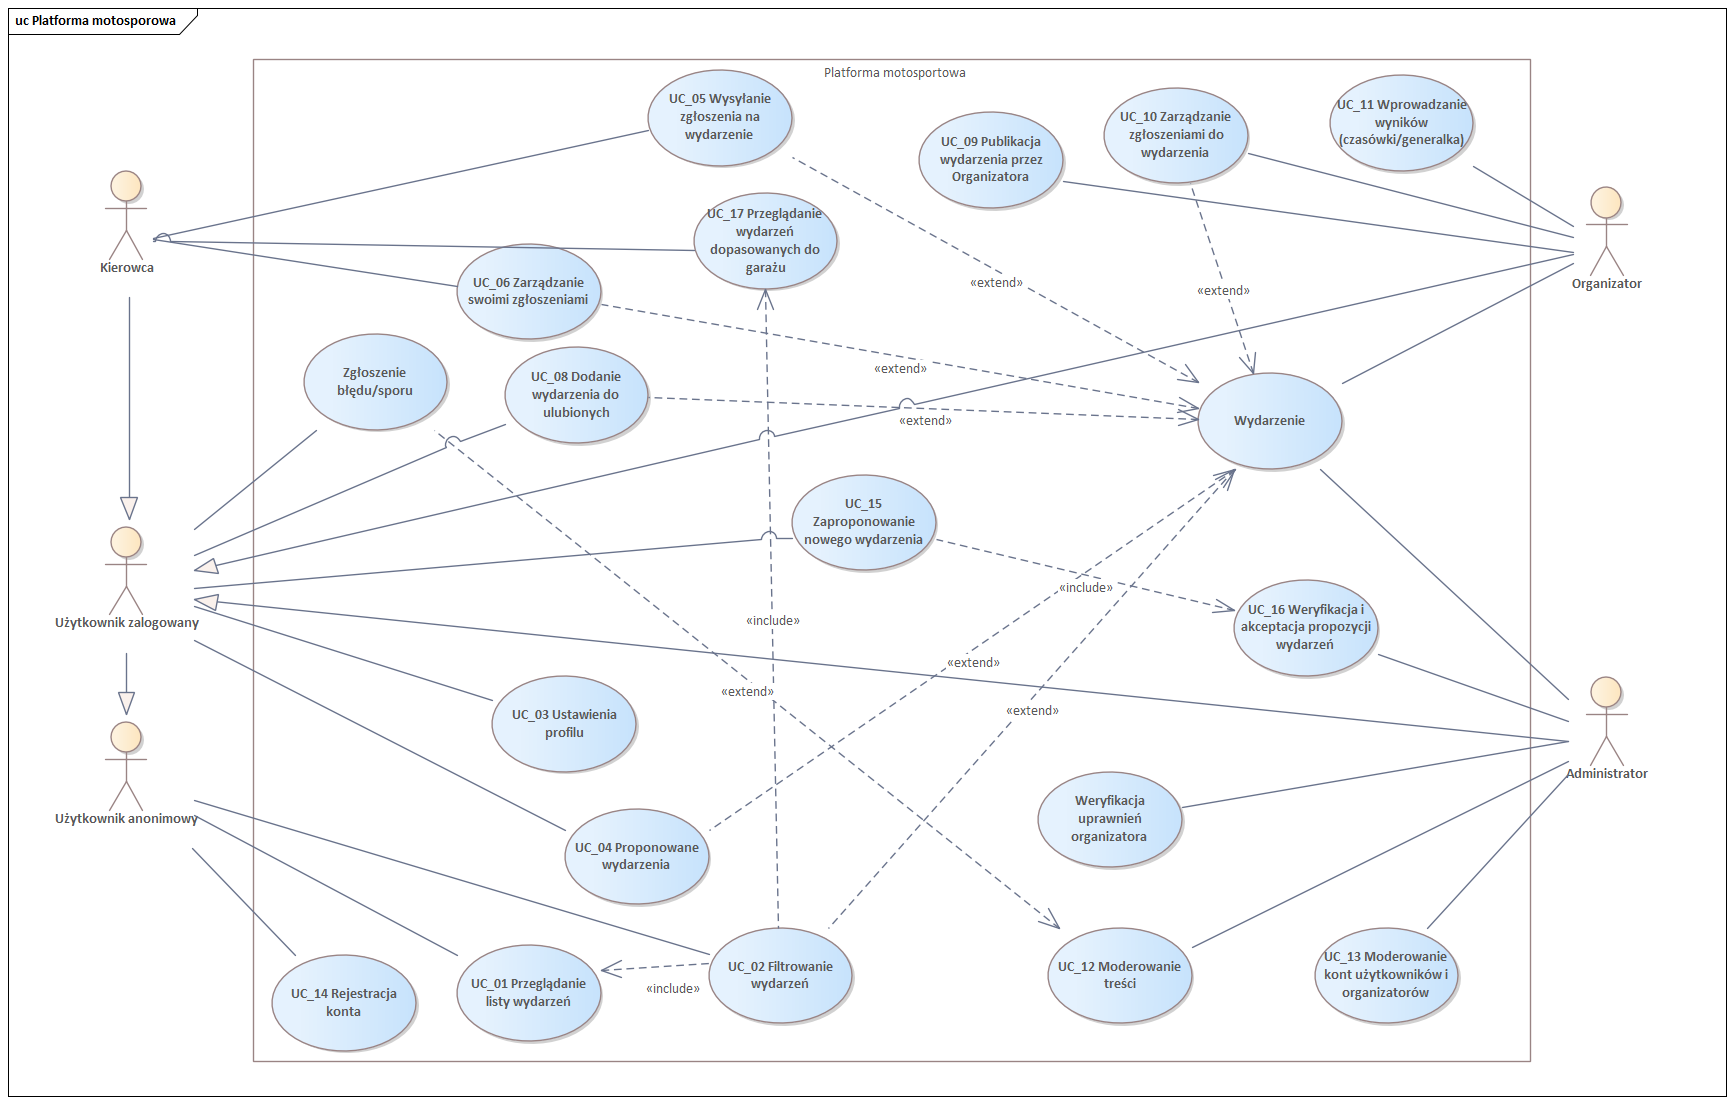
\includegraphics[width=\textwidth]{platforma-motorsportowa.png}
  \caption{Diagram przypadków użycia --- Platforma motorsportowa (wersja koncepcyjna).}
  \label{fig:use-case}
\end{figure}

\subsection{Diagram sekwencji: rejestracja i logowanie}
% TODO: wstawić diagram sekwencji
\subsection{Diagram sekwencji: zapis na wydarzenie}
% TODO
\subsection{Diagram sekwencji: zarządzanie garażem}
% TODO

\noindent\textit{Uwaga:} diagram klas / model danych przeniesiono do projektu systemu --- podrozdział~\ref{sec:diagram-klas}.

\chapter{Projekt systemu}
\label{ch:projekt}
\section{Założenia architektoniczne}
Architektura trójwarstwowa: klienty (web, mobile) $\rightarrow$ API REST $\rightarrow$ MySQL. Statyczny frontend za nginx z~proxy \texttt{/api}.

\section{Architektura logiczna systemu}
Moduły domenowe: użytkownicy/auth, wydarzenia, zgłoszenia, garaż, organizator, administracja, mapy/trasa, poczta.

\section{Architektura fizyczna i wdrożeniowa}
\label{sec:arch-fizyczna}
Kontenery lokalne: \texttt{web}, \texttt{api}, \texttt{mysql}, \texttt{mailhog} (Mailpit), \texttt{backup}. Mobile poza Compose.

Wdrożenie produkcyjne: maszyna Oracle Always Free (ARM) z~Docker Compose; publiczny dostęp przez \textbf{Cloudflare Tunnel} (\texttt{cloudflared}) do nginx na porcie \texttt{:8081}. Domena \url{https://raceportal.pl} jest w~tym samym koncie Cloudflare --- TLS i~DNS po stronie Cloudflare, bez hostowania frontu na Cloudflare Pages. Maile produkcyjne: SMTP Mailbux.

\section{Projekt bazy danych}
Encje m.in.: użytkownik, pojazd, wydarzenie, zgłoszenie, wniosek organizatora; statusy wydarzeń i~zgłoszeń; współrzędne geograficzne wydarzenia.

\subsection{Diagram klas}
\label{sec:diagram-klas}
Rysunek~\ref{fig:diagram-klas} przedstawia wczesny model bazy danych (ERD) stanowiący punkt wyjścia projektu klas / tabel domenowych. W~implementacji Spring Data JPA model został uproszczony i~dostosowany do MVP (m.in.\ role jako enum użytkownika, lokalizacja osadzona w~wydarzeniu).

\begin{figure}[ht]
  \centering
  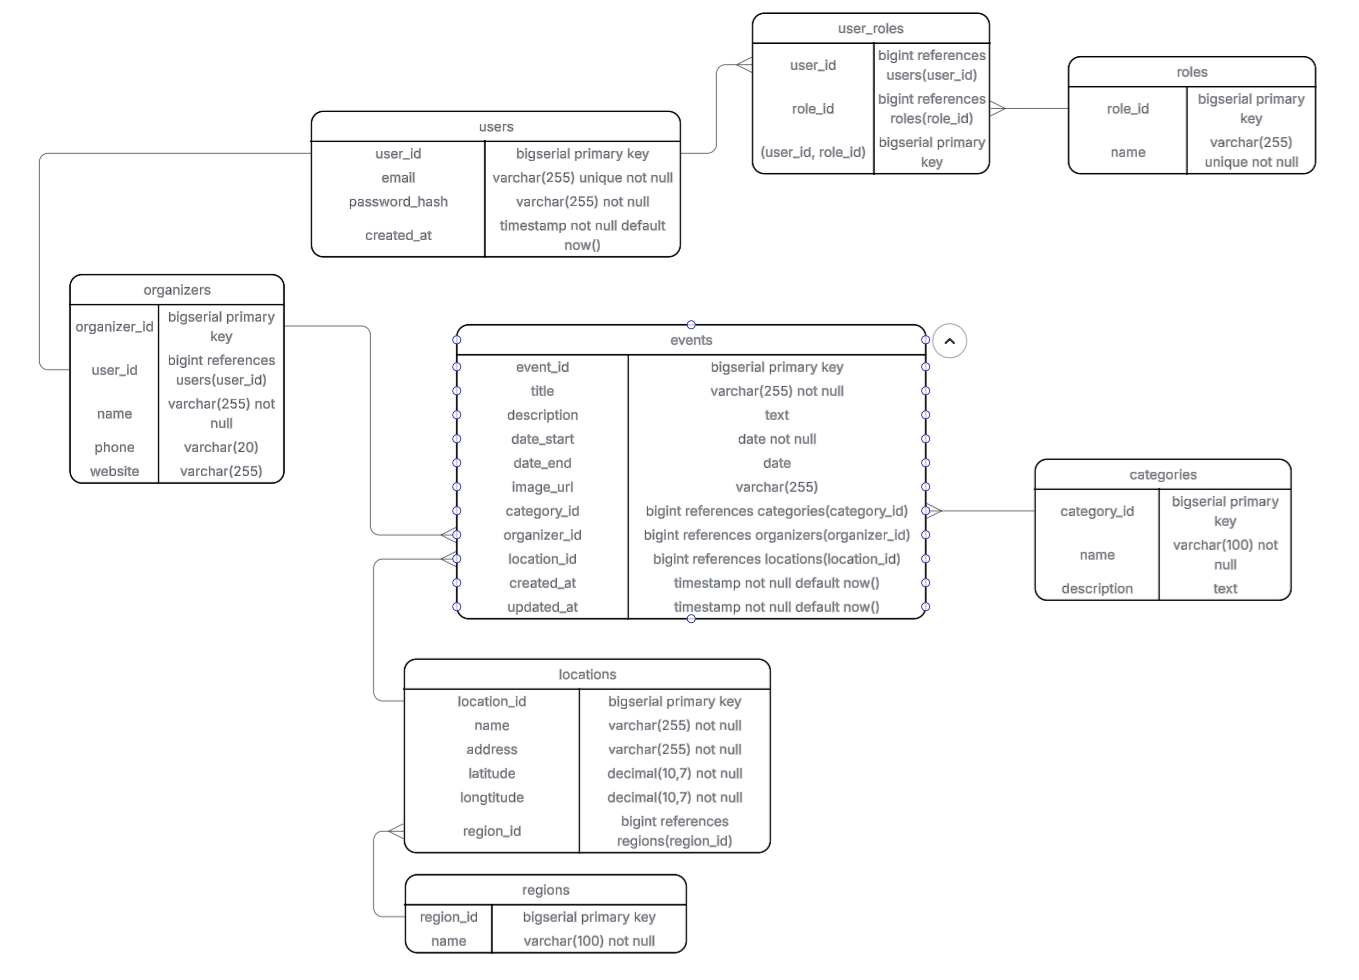
\includegraphics[width=\textwidth]{model-bazy-danych.png}
  \caption{Diagram klas / model danych (ERD) --- wersja koncepcyjna projektu.}
  \label{fig:diagram-klas}
\end{figure}

\section{Projekt interfejsu REST API}
Zasoby \texttt{/api/auth/*}, \texttt{/api/events}, \texttt{/api/events/markers}, \texttt{/api/registrations}, \texttt{/api/garage}, \texttt{/api/admin/*}, \texttt{/api/organizer/*}, \texttt{/api/maps/route}, \texttt{/api/health}.

\section{Projekt warstwy webowej}
\label{sec:figma}
Routing React Router; AuthContext; strony katalogu, detalu, dashboardu, garażu, paneli; komponent mapy Leaflet.

\subsection{Prototyp UI w~Figma Make}
Wyjściowym projektem interfejsu był plik Figma Make \textbf{Advanced UI/UX for RACEPORTAL} (ciemny motyw motorsportowy, akcent marki, Orbitron / typografia display, komponenty zbliżone do shadcn/ui). Prototyp obejmował m.in.\ stronę główną, katalog, logowanie/rejestrację, dashboard oraz szkice paneli organizatora i~administratora.

Kod frontendu został przeniesiony z~Figma Make do lokalnego monorepo (Vite/React), a~następnie podpięty pod realne API (zamiast mocków / localStorage). Wczesna wizja produktu i~ról --- jeszcze przed pełną implementacją --- jest też widoczna na diagramach koncepcyjnych (rys.~\ref{fig:use-case}, \ref{fig:podzial-rol}).

W~toku realizacji UI dopracowano pod kątem responsywności, stanów pustych/błędów, PWA (manifest, service worker, dolna nawigacja mobilna) oraz spójności z~tokenami marki (\texttt{--race-accent}).

\section{Projekt aplikacji mobilnej}
Stack Expo; nawigacja stack Eventy; publiczny klient HTTP; \texttt{EXPO\_PUBLIC\_API\_URL} / \texttt{EXPO\_PUBLIC\_WEB\_URL}; CTA \texttt{Linking} do \texttt{/wydarzenia/:id}.

\section{Projekt mechanizmów bezpieczeństwa}
JWT w~nagłówku Authorization (web); role na endpointach; walidacja DTO; CORS; CSP nginx.

\chapter{Realizacja}
\section{Organizacja implementacji}
Implementacja iteracyjna w~monorepo, z~dokumentowaniem zmian i~utrzymywaniem środowiska Compose jako źródła prawdy uruchomieniowej.

\section{Podział systemu na komponenty}
\subsection{Backend}
Spring Boot: kontrolery, serwisy, repozytoria JPA, seed (\texttt{DataInitializer}), joby (np.\ archiwizacja).
\subsection{Frontend webowy}
Vite + React; integracja z~API; stany ról i~formularze dziedzinowe.
\subsection{Aplikacja mobilna}
Expo --- katalog publiczny bez auth.
\section{Integracja komponentów}
Wspólny kontrakt JSON; typy w~\texttt{api-types}; nginx reverse proxy \texttt{/api} w~środowisku Compose.
\section{Konteneryzacja i uruchamianie środowiska}
\texttt{docker compose up --build -d}; weryfikacja \texttt{/api/health}; Expo: \texttt{cd mobile \&\& npm start}. Publiczny dostęp produkcyjny: Cloudflare Tunnel $\rightarrow$ nginx \texttt{:8081}.

\chapter{Szczegóły implementacji backendu}
\label{ch:backend}
\section{Struktura projektu backendowego}
Pakiet \texttt{pl.raceportal} --- warstwy controller / service / repository / dto / security.
\section{Model domenowy i encje}
Użytkownik (role), Car, Event, Registration oraz powiązane statusy i~flagi wymagań wydarzenia.
\section{Rejestracja użytkowników i logowanie}
Rejestracja z~opcjonalną weryfikacją e-mail (kod); logowanie hasłem; opcjonalna wymiana Google idToken $\rightarrow$ JWT.
\section{Zarządzanie profilami użytkowników}
Aktualizacja danych profilu, hasła, deklaracji (m.in.\ PZM, prawo jazdy B), pól adresu / Instagram.
\section{Obsługa wydarzeń}
Listowanie z~filtrami i~paginacją; markery mapy; CRUD po stronie organizatora; moderacja admina; archiwum.
\section{Obsługa zgłoszeń}
Tworzenie zgłoszenia z~wyborem pojazdu; walidacja wymagań; zmiana statusów; anulowanie; maile transactional.
\section{Obsługa garażu}
CRUD pojazdów; reguły clear-on-edit pól liczbowych; powiązanie z~kategorią wydarzenia.
\section{Panel administratora i organizatora}
Endpointy i~reguły RBAC dla moderacji i~zarządzania zgłoszeniami / wydarzeniami.
\section{Integracja z bazą danych}
Spring Data JPA + MySQL 8; konfiguracja przez zmienne środowiskowe Compose.
\section{Obsługa wyjątków i walidacja}
Bean Validation; odpowiedzi z~polem \texttt{details}; mapowanie na komunikaty UI.

\chapter{Szczegóły implementacji frontendu webowego}
\label{ch:frontend}
\section{Struktura aplikacji webowej}
Katalog \texttt{web/src/app}: \texttt{pages/}, \texttt{components/}, \texttt{context/}, \texttt{lib/}.
\section{Strona główna i katalog wydarzeń}
Widoki Lista / Mapa / Kalendarz; debounce filtrów; „Wyczyść filtry”; paginacja listy vs markery overview.
\section{Widok szczegółów wydarzenia}
Opis, wymagania, zapis z~wyborem auta, \texttt{carMatch}, mapa i~trasa.
\section{Logowanie i rejestracja}
Formularze auth; weryfikacja kodu; reset hasła; opcjonalny Google Sign-In.
\section{Dashboard użytkownika}
Zgłoszenia użytkownika i~szybkie informacje o~nadchodzących startach.
\section{Widok garażu}
Formularz pojazdu, walidacja pól wymaganych, edycja i~usuwanie (z~ograniczeniami przy otwartym zgłoszeniu).
\section{Panel organizatora}
Tworzenie/edycja wydarzeń, lista zgłoszeń, zmiana statusów.
\section{Panel administratora}
Moderacja wydarzeń, wnioski organizatora, zarządzanie rolami.
\section{Mapa i elementy lokalizacyjne}
Leaflet + kafelki CARTO; pickery lokalizacji; proxy trasy \texttt{/api/maps/route}.
\section{Responsywność i doświadczenie użytkownika}
Układ dostosowany do desktop/mobile web; motyw z~akcentem \texttt{--race-accent}.

\chapter{Szczegóły implementacji aplikacji mobilnej}
\section{Założenia aplikacji mobilnej}
Mobilka ma wspierać odkrywanie wydarzeń, a~nie dublować pełnego klienta webowego.
\section{Architektura rozwiązania mobilnego}
Expo SDK, React Navigation (stack Eventy), ThemeProvider, cienki klient API bez JWT.
\section{Lista wydarzeń i widok szczegółów}
Filtry publiczne; przełączanie Lista / Kalendarz / Mapa; detal z~metadanymi wydarzenia.
\section{Nawigacja i interfejs użytkownika}
Pojedynczy stack: \texttt{EventsList} $\rightarrow$ \texttt{EventDetail}; dark UI spójny z~marką.
\section{Integracja z API}
Publiczne GET (events, markers, health); konfiguracja hosta API (localhost / LAN / Android emulator).
\section{Przekierowanie do wersji webowej}
Przycisk „Zapisz się na stronie” --- \texttt{Linking.openURL(webEventUrl(id))}.
\section{Ograniczenia wersji mobilnej}
Brak auth, garażu, paneli ról i~archiwum w~aplikacji; zależność od dostępności weba przy konwersji zapisu.

\chapter{Bezpieczeństwo systemu}
\label{ch:bezpieczenstwo}
\section{Założenia bezpieczeństwa}
Ochrona kont i~danych zgłoszeń na poziomie ASVS L1 adekwatnym do MVP demonstracyjnego.
\section{Klasyfikacja danych}
Dane konta i~profilu; dane pojazdów; dane zgłoszeń; treści wydarzeń (częściowo publiczne).
\section{Uwierzytelnianie użytkowników}
Hasło + JWT; opcjonalnie Google; brak sesji serwerowej klasycznej.
\section{Autoryzacja i kontrola dostępu RBAC}
Role USER / ORGANIZER / ADMIN egzekwowane w~API i~bramkach UI.
\section{Wykorzystanie tokenów JWT}
Token przechowywany po stronie klienta web; dołączany do żądań chronionych.
\section{Walidacja danych wejściowych}
Walidacja DTO po stronie API; walidacja formularzy UI; komunikaty pól \texttt{details}.
\section{Ochrona zasobów użytkowników}
Dostęp do garażu i~zgłoszeń wyłącznie właściciela (oraz uprawnionych ról w~panelach).
\section{Bezpieczeństwo komunikacji}
W~dev HTTP lokalne; w~prod TLS terminowany na Cloudflare Tunnel przed nginx; CSP / X-Frame-Options na nginx.
\section{Analiza zagrożeń}
Uwierzytelnianie, IDOR, XSS, CSRF w~kontekście SPA, brute-force logowania (rate limit).
\section{Analiza ryzyka}
Ryzyko akceptowalne dla środowiska demo; produkcja wymaga twardego sekretu JWT, HTTPS i~polityki haseł zsynchronizowanej backend$\leftrightarrow$UI.
\section{Ograniczenia przyjętych zabezpieczeń}
Brak 2FA; Google OAuth opcjonalny; brak WAF; publiczny OSRM bez SLA.

\chapter{Testowanie i weryfikacja systemu}
\label{ch:testy}
\section{Strategia testowania}
Piramida: unit (api-types, mobile client) $\rightarrow$ integracyjne API (MockMvc) $\rightarrow$ E2E Playwright (web + preview mobile).
\section{Środowisko testowe}
Docker Compose + opcjonalnie Expo web \texttt{:8082}; dokumentacja \texttt{docs/testy/TESTY.md}.
\section{Testy jednostkowe}
Vitest: \texttt{packages/api-types}, \texttt{mobile/tests}.
\section{Testy integracyjne backendu}
JUnit / MockMvc --- scenariusze auth, eventy, garaż, zgłoszenia, RBAC, trasa.
\section{Testy End-to-End aplikacji webowej}
Playwright: ścieżki katalogu, auth, garaż, role (viewport desktop/mobile).
\section{Testy aplikacji mobilnej}
Unit URL API/WEB; E2E gość (lista, widoki, detal, CTA) na Expo web.
\section{Testy mechanizmów bezpieczeństwa}
Scenariusze braku dostępu do paneli obcych ról; walidacja wejścia.
\section{Automatyzacja uruchamiania testów}
Skrypty npm / \texttt{scripts/}; raporty w~\texttt{docs/testy/wyniki/}.
\section{Analiza wyników testów}
Werdykty przebiegów odnotowywane w~dokumentacji wyników; regresie łapane przed prezentacją.
\section{Ograniczenia procesu testowania}
Brak pełnych testów natywnych (Detox/Maestro); \textbf{brak formalnego load testu 10k rekordów / 50~RPS} w~MVP --- ograniczenie omówione w~podsumowaniu.

\chapter{Prezentacja systemu}
\section{Prezentacja głównych funkcjonalności}
Demonstracja katalogu (3 widoki), zapisu kierowcy z~\texttt{carMatch}, paneli org/admin oraz mobile CTA --- zgodnie z~\texttt{docs/scenariusz-prezentacji.md}.
\section{Scenariusz użycia z perspektywy kierowcy}
Login seed $\rightarrow$ garaż $\rightarrow$ filtr/katalog $\rightarrow$ zapis $\rightarrow$ dashboard statusów.
\section{Scenariusz użycia z perspektywy organizatora}
Login org $\rightarrow$ wydarzenie $\rightarrow$ zgłoszenia $\rightarrow$ zmiana statusu $\rightarrow$ podgląd maila w~Mailpit.
\section{Scenariusz użycia z perspektywy administratora}
Login admin $\rightarrow$ moderacja wydarzenia / wniosku organizatora / ról.
\section{Podsumowanie działania systemu}
System realizuje spójny obieg informacji o~wydarzeniach i~zapisach w~środowisku uruchamialnym lokalnie oraz pod adresem produkcyjnym za Cloudflare Tunnel.

\chapter{Nakład pracy}
\section{Liczba godzin przeznaczona na realizację projektu}
% TODO: wpisać sumaryczny nakład (osobogodziny)
\section{Podział zadań w zespole}
Skrót obszarów --- rozdz.~\ref{ch:wklad}. Szczegółowa tabela godzin: TODO.
\section{Narzędzia wspierające zarządzanie pracą}
Git/GitHub, dokumentacja Markdown w~\texttt{docs/}, Docker, Cursor/IDE, Playwright, Figma Make, Cloudflare Dashboard.
\section{Problemy organizacyjne i ich rozwiązanie}
M.in.\ rozrost zakresu mobile --- decyzja o~wizytówce; luki Spec --- rejestr \texttt{spec-conformity.md}; stabilizacja testów względem seedu/archiwizacji; uproszczenie hostingu (Oracle + Tunnel zamiast GCP Pages).

\chapter{Wkład własny}
\label{ch:wklad}
Rozdział opisuje, kto odpowiadał za które obszary prac projektowych i~implementacyjnych (imię i~nazwisko). Podział odzwierciedla faktyczny udział zespołu; największy wkład merytoryczny i~projektowy w~warstwie produktu/UI wniosła Natalia Otrombke.

\section{Natalia Otrombke}
\begin{itemize}
  \item projekt UI/UX w~Figma Make (\textbf{Advanced UI/UX for RACEPORTAL}) --- ekrany katalogu, auth, dashboard, paneli;
  \item przeniesienie i~dopracowanie frontendu React (motyw, layout, spójność marki, kluczowe ścieżki UX);
  \item udział w~definicji flow użytkownika (gość $\rightarrow$ kierowca $\rightarrow$ organizator) oraz w~materiałach koncepcyjnych ról.
\end{itemize}

\section{Oliwier Kasprowicz}
\begin{itemize}
  \item prace analityczne i~dokumentacyjne (wymagania, prezentacje zespołowe);
  \item wsparcie przy diagramach i~scenariuszach użycia;
  \item udział w~przeglądach zakresu MVP i~odbiorze funkcjonalności.
\end{itemize}

\section{Michał Gutowski}
\begin{itemize}
  \item diagramy i~materiały projektowe (m.in.\ rich picture, przepływy);
  \item wsparcie dokumentacji i~testów scenariuszy prezentacji;
  \item udział w~integracji i~weryfikacji ścieżek użytkownika.
\end{itemize}

\section{Miłosz Parkitny}
\begin{itemize}
  \item modelowanie i~diagramy (m.in.\ przypadki użycia, podział funkcjonalności, model danych);
  \item wsparcie analizy interesariuszy i~harmonogramów;
  \item udział w~pracach implementacyjnych / poprawkach w~repozytorium.
\end{itemize}

\section{Wojciech Wronisz}
\begin{itemize}
  \item backend Spring Boot (API, JWT/RBAC, encje, seed, maile);
  \item Docker Compose, wdrożenie produkcyjne Oracle + \textbf{Cloudflare Tunnel}, Mailbux, PWA;
  \item dokumentacja uruchomienia i~odbioru (\texttt{docs/}), testy API / E2E, integracja web~$\leftrightarrow$~API.
\end{itemize}

\chapter{Podsumowanie}
\label{ch:podsumowanie}
\section{Największe wyzwania i sposób ich rozwiązania}
Spójność domeny zapisów i~garażu, RBAC, mapa/trasa oraz utrzymanie monorepo web+API+mobile. Po stronie infrastruktury --- uproszczenie hostingu do jednej VM z~tunelowaniem Cloudflare zamiast rozdzielonego stacku Pages/Worker.

\section{Zmiany i adaptacje w trakcie realizacji}
Przejście mobile z~parity na wizytówkę; doprecyzowanie formularzy; wspólny pakiet typów; migracja z~eksperymentów GCP/Pages na Oracle + Cloudflare Tunnel.

\section{Ograniczenia końcowej wersji systemu}
Brak PSP i~uploadu plików; mobilka bez konta; limity testów wydajnościowych i~produkcyjnego hardeningu.

\subsection{Ograniczenia wydajnościowe (RPS)}
W~wymaganiach jakościowych MVP zapisano docelowy test obciążenia: \textbf{ok.\ 10\,000 rekordów} w~katalogu oraz \textbf{ok.\ 50~RPS} przy akceptowalnym P95 odpowiedzi list/detalu. W~oddawanej wersji:
\begin{itemize}
  \item zastosowano mitigacje lokalne (paginacja listy, osobne markery mapy, indeksy / cache tam gdzie uzasadnione);
  \item \textbf{nie wykonano} formalnego load testu 10k/50~RPS (brak raportu RPS/P95 jako artefaktu odbioru);
  \item środowisko produkcyjne (Oracle Always Free + Cloudflare Tunnel) jest wystarczające do demonstracji i~ruchu prezentacyjnego, ale nie zostało zweryfikowane pod kątem założonego progu 50~RPS.
\end{itemize}
Ograniczenie to jest świadome: priorytetem było domknięcie happy-path funkcjonalnego, bezpieczeństwa podstawowego (JWT/RBAC) i~uruchamialności. Pomiar 10k/50~RPS pozostaje w~backlogu jakościowym.

\section{Możliwości dalszego rozwoju}
Płatności, upload, watchlista, iCal, waitlista, eksport list startowych, store/PWA --- por.\ \texttt{docs/pomysly-rozwoju.md}; uzupełnienie testów obciążeniowych RPS.

\section{Wnioski końcowe}
RacePortal stanowi kompletne MVP demonstracyjne katalogu i~zapisów motorsportowych z~czytelnością architektury, testami funkcjonalnymi i~ścieżką prezentacji dla odbiorcy akademickiego oraz biznesowego --- przy jasno nazwanych lukach (PSP, upload, load test RPS).

\printbibliography[title={Bibliografia}, heading=bibintoc]

\clearpage
\phantomsection
\addcontentsline{toc}{chapter}{Spis rysunków}
\listoffigures

\clearpage
\phantomsection
\addcontentsline{toc}{chapter}{Spis tabel}
\listoftables

\makethesisattachments

\end{document}
